\begin{figure}[htb!]
\centering
\begin{tabular}{ccc}
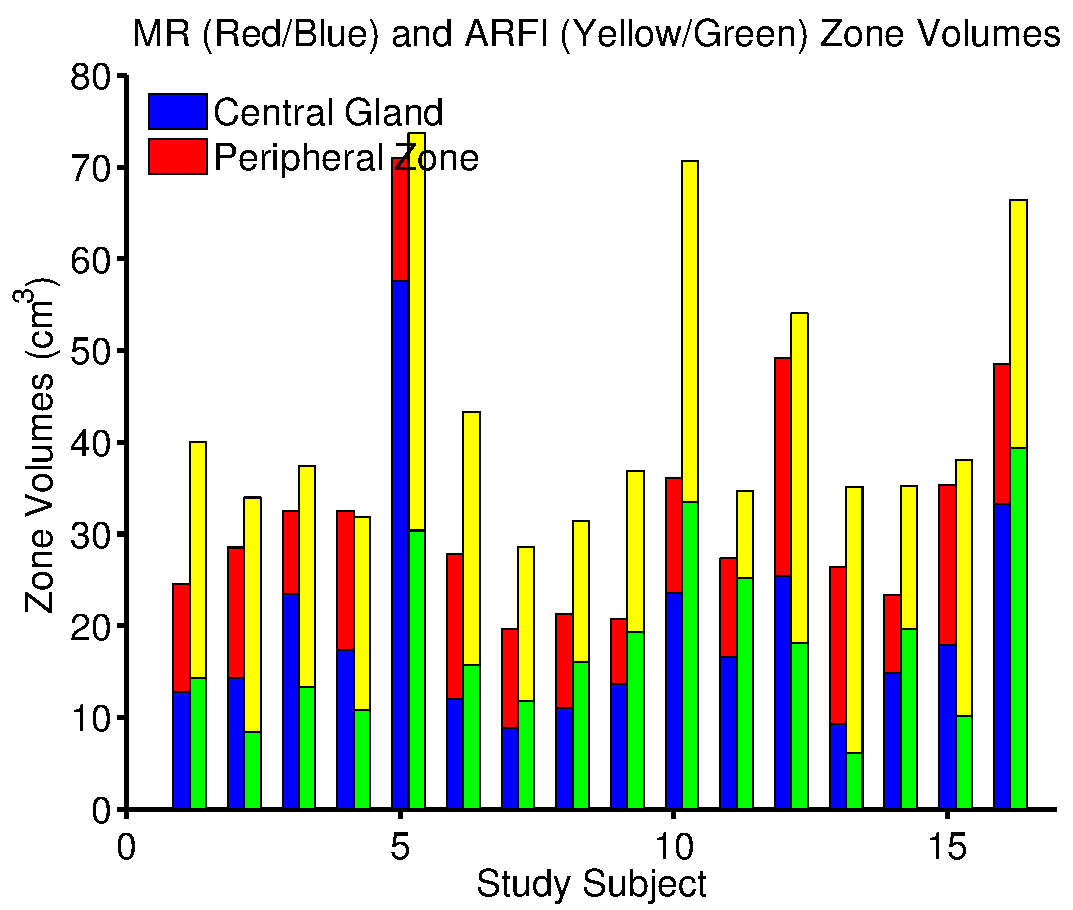
\includegraphics[width=0.3\linewidth]{figs/mr_arfi_volumes.pdf} &
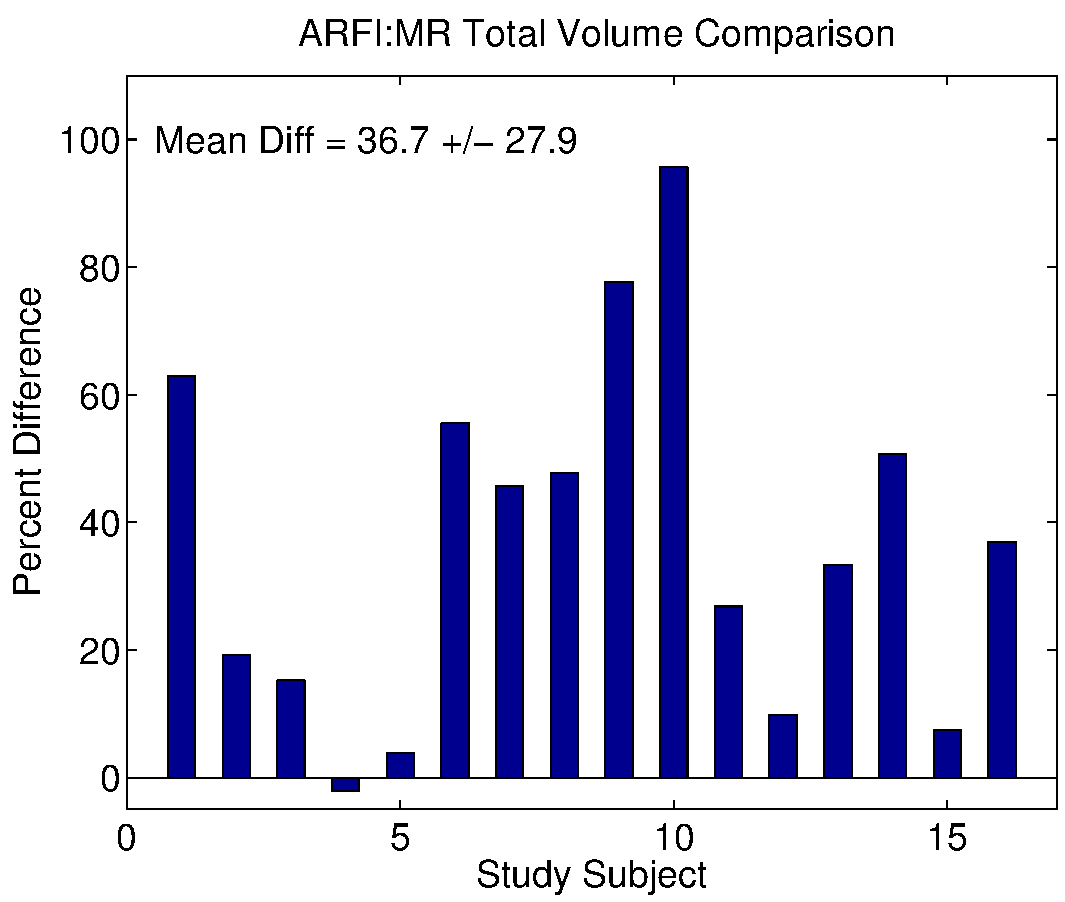
\includegraphics[width=0.3\linewidth]{figs/mr_arfi_volume_diff.pdf} &
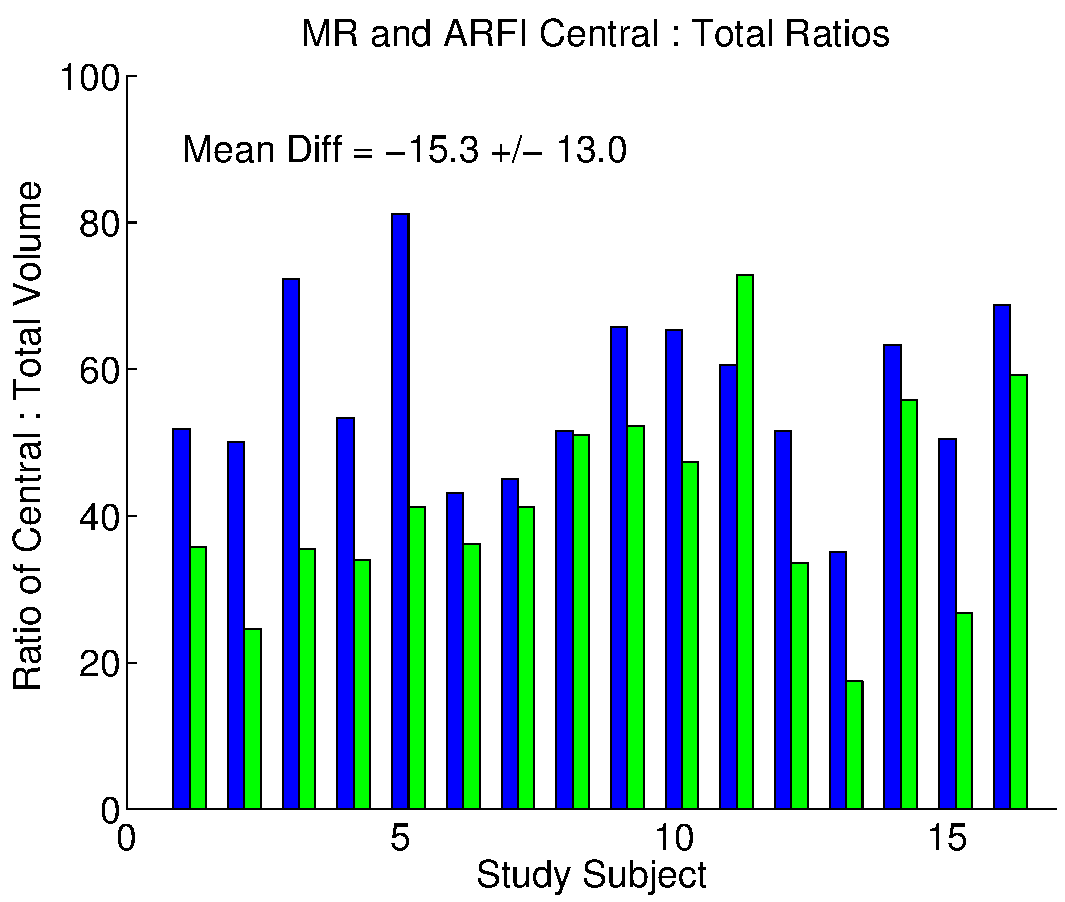
\includegraphics[width=0.3\linewidth]{figs/mr_arfi_central_total_diff.pdf} \\
(a) Central:Peripheral Volume & (b) Total Volume Difference & (c) Central:Total Volume Difference\\
\end{tabular}
\caption{Comparison of MR and ARFI zonal anatomy volume estimates from manually-segmented images.  Total prostate volumes ranged from 19.6--71.0 cm$^3$ based on MR image models (a), with ARFI image models overestimating total prostate volume by 36.7 $\pm$ 27.9\% (b).  ARFI image delineation of the central zone volume relative to total prostate volume showed a mean underestimation of -15.3 $\pm$ 13.0\% (c, green) relative to the MR central gland : total volume ratios (c, blue).}
\label{fig:mr_arfi_volumes} 
\end{figure}
